\subsubsection{Activity Diagrams}
Activity diagrams are employed to give insights to the reader about specific sequences of operations occurring in some parts of the system being described.
In this case, they illustrate the procedures actuated to calculate the score of a code solution submitted through GitHub and to terminate a battle.  \\

\begin{minipage}{\linewidth}
	\textbf{Computing Score}\\
	
	
	\begin{center}
		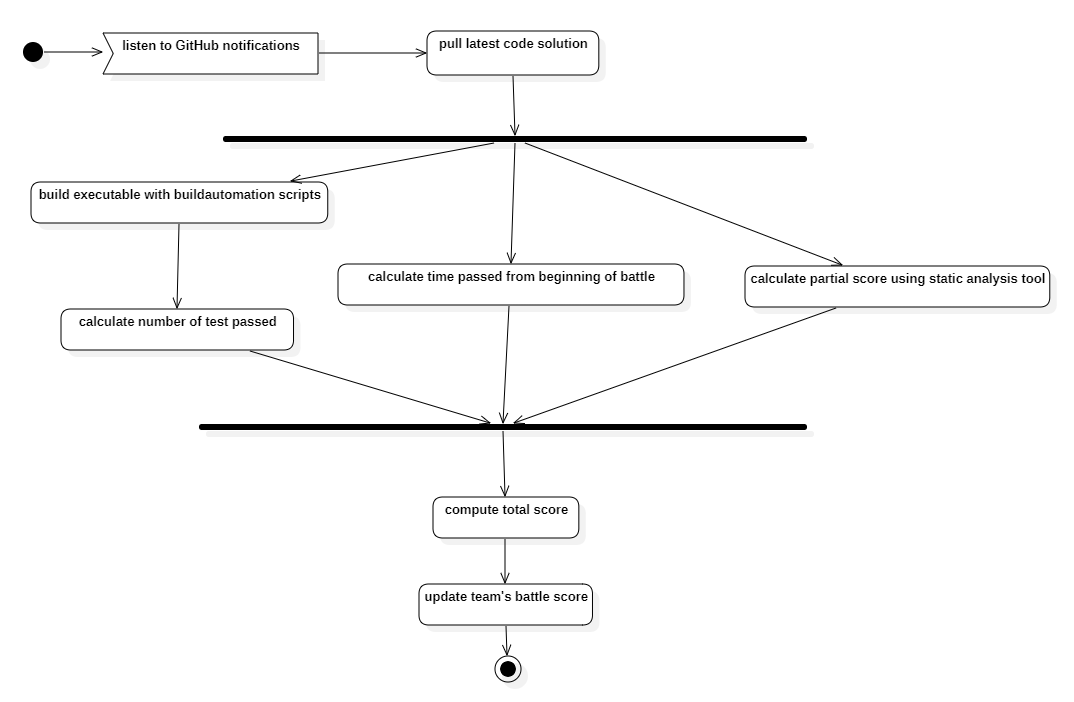
\includegraphics[width=1\textwidth]{3Specific_Requirements/res/ActivityDiagramCalculateScore}
	\end{center}
\end{minipage}

The first activity diagram regards the process for computing the score of a code solution to a battle submitted by a student through GitHub. The procedure is initiated when a new commit is pushed by a student in the main branch of his forked GitHub repository. GitHub sends a notification to \app, which causes the system to download the latest code solution. Since the final score is obtained by combining results of three different analyses (static analysis, timeliness and number of test cases passed) the diagram shows how these three computations are carried out in parallel.

\newpage

\textbf{TerminateBattle}\\
\begin{figure}[h]
	\centering
	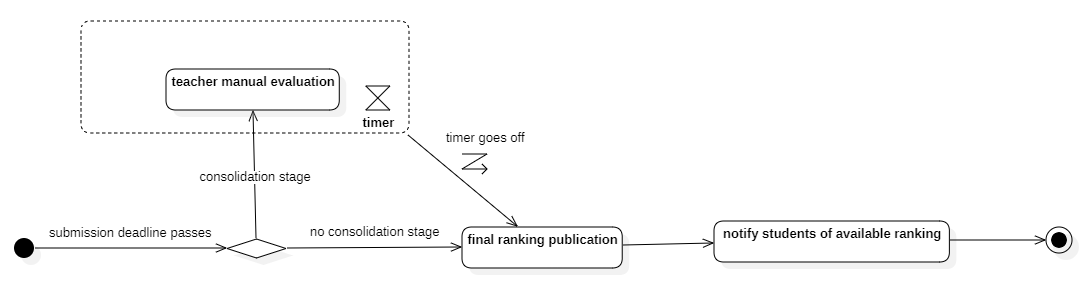
\includegraphics[width=1\textwidth]{3Specific_Requirements/res/ActivityDiagramTerminateBattle}
\end{figure}

This activity diagram delineates the process that leads to terminating a battle and publish the conclusive battle results. The procedure is initiated upon the expiration of the battle submission deadline. The diagram is of interest because it highlights the workflow of when a battle expects a manual evaluation. The  \textbf{manual evaluation} activity is executed by an educator. If this activity doesn't terminate before the time set by the timer, the system autonomously proceeds ignoring the consolidation stage scores and publishing the final ranking based on the scores assigned during the battle.